\subsection{Visualization}
A usefull way debug \gs applications is to generate visualizations of the pipeline.
To acheive this the environe ment variable \code{GST_DEBUG_DUMP_DOT_DIR} must be defined and the \code{GST_DEBUG_BIN_TO_DOT_FILE} macro needs to be executed on the final graph if it is part of a custom GStreamer application, whic is the case on the \sr.
\cite{johnstonGeneratingGStreamerPipeline2018}
This will generate temprorary information \textit{.dot} files that can later be converted to visualized graphs using \gls{gviz}.
Figure \ref{fig:gs_pipeline_visualization} shows the final graph that is used on the \sr.
It has been modified in Adobe Illustrator to be more compact, but is still to large to b




\begin{figure}[H]
    \centering
    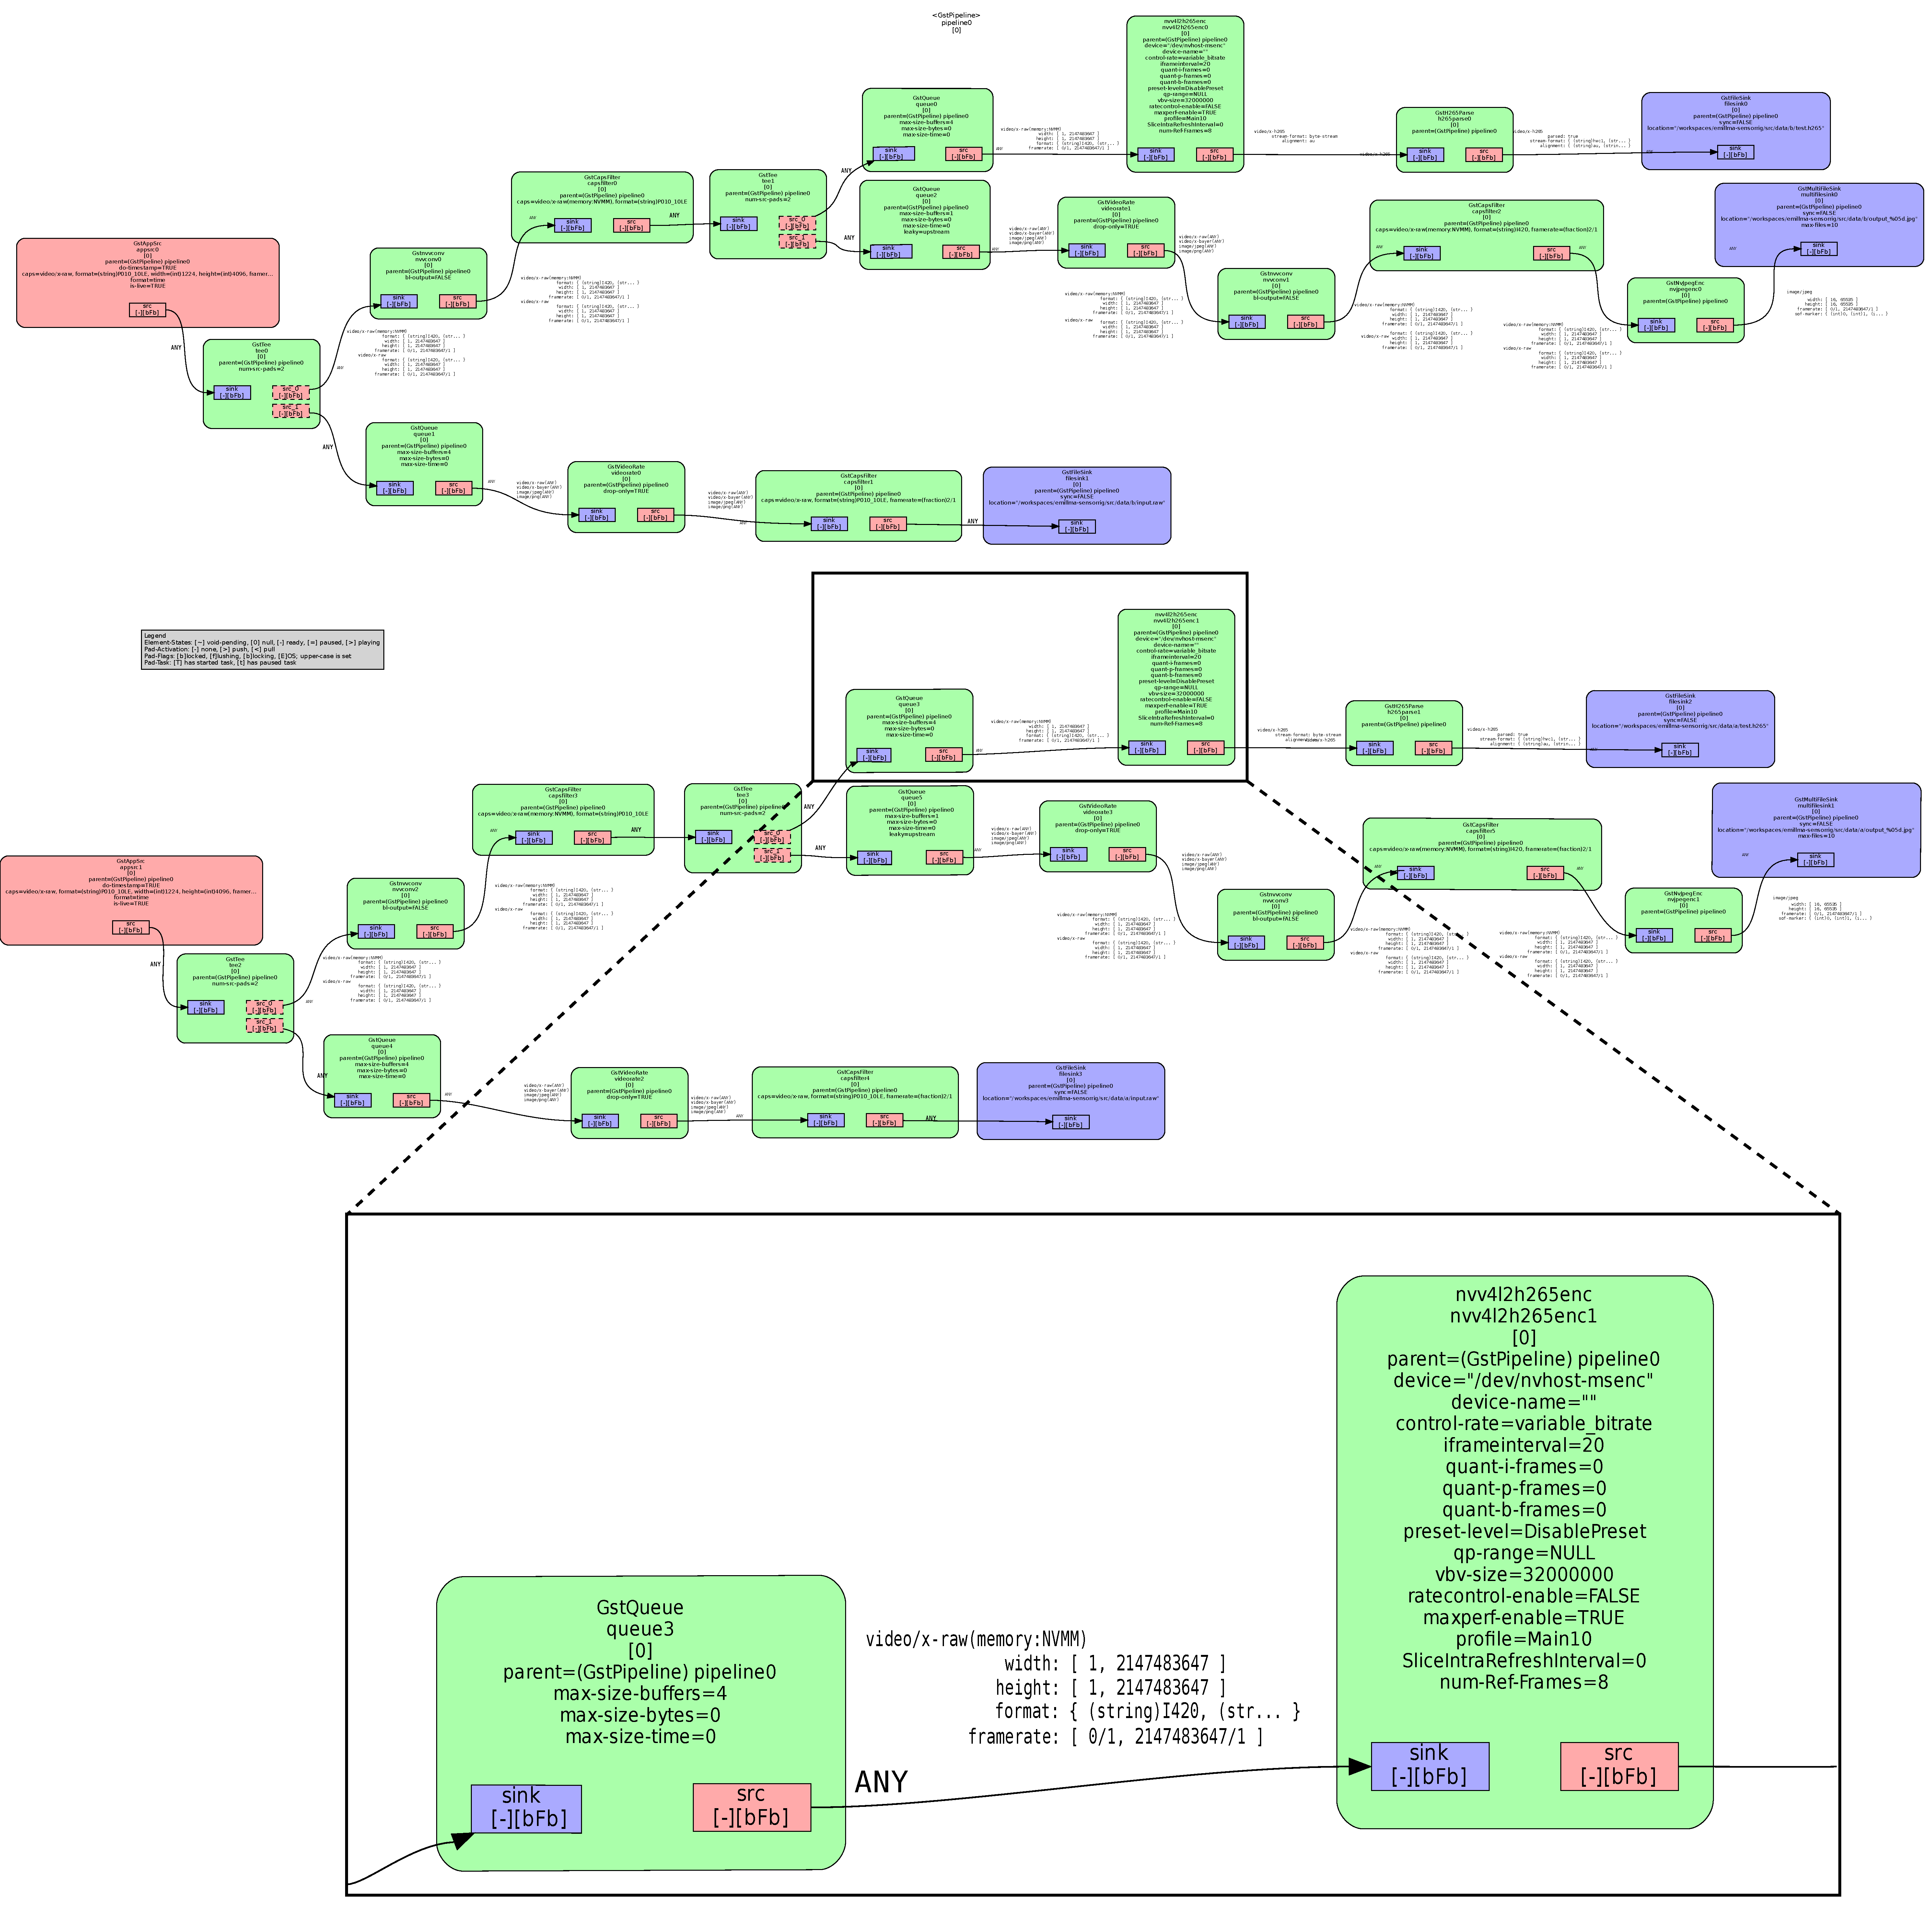
\includegraphics[width=\textwidth]{figures/pipeline.pdf}
    \caption{Visualization of the \gs Pipeline used on the \sr.
        The graph was crated using GraphViz and edited in Adobe Illustrator to be more compbact and readable. The bottom part shows a zoomed in version of the encoder part of used on the second camera.}
    \label{fig:gs_pipeline_visualization}
\end{figure}